\documentclass[a4paper,11pt]{article}
\usepackage[utf8]{inputenc}
\usepackage[T1]{fontenc}
\usepackage[magyar]{babel}
\usepackage{indentfirst}
\usepackage{graphicx}
\usepackage[export]{adjustbox}
\usepackage[final]{pdfpages}
\frenchspacing
\author{Géczi Péter}
\title{
		Kutatómunka információs eszközei \\
		\textbf{Müon részecskék becsapódásának időbeli eloszlása}}
\date{2017. május 28.} 
\begin{document}
\maketitle
\pagebreak

\section{A probléma ismertetése}
A müonokat a kozmikus sugárzás révén detektálhatjuk a Földön, ezek a részecskék anyagban elnyelődnek és szóródnak. A müonokat, egy úgynevezett gáztöltésű detektorral detektáltuk. Egy ilyen detektor több, egymásra helyezett, párhuzamos lapból áll. Amikor áthalad rajtuk egy müon, a lapok, megfelelő szálain feszültség keletkezik, így egy háromdimenziós képet kaphatunk a részecske detektoron belüli pályájáról. Egy ilyen megszólalást nevezhetünk eseménynek, ez a felhasznált adatfájl egy sorát teszi ki. A részecske pozícióin és a detektor egyéb adatain kívül, egy esemény tartalmazza az előző esemény óta eltelt időt $\mu s$-ban, a jegyzőkönyv célja, hogy ennek az eloszlását elemezze.
\newline
Egy ilyen valós mérés eredményeit tartalmazza a 'bemenet.txt' fájl, összesen 10000 eseménnyel. Minden sor 2. oszlopa az előző esemény óta eltelt idő $\mu s$-ban. A bemenetet egy C++-ban írt kód segítségével beolvastam, majd az adatokból két különböző paraméterű hisztogramot készítettem, a hisztogramok adatait kiírattam a 'histogram\_out1.txt' és 'histogram\_out2.txt' fájlokba.

\section{Eredmény}
A program kimenetét gnuplottal ábrázoltam.
\newline
Egy kisebb binméretű hisztogram:

\begin{figure}[h]
{\centering 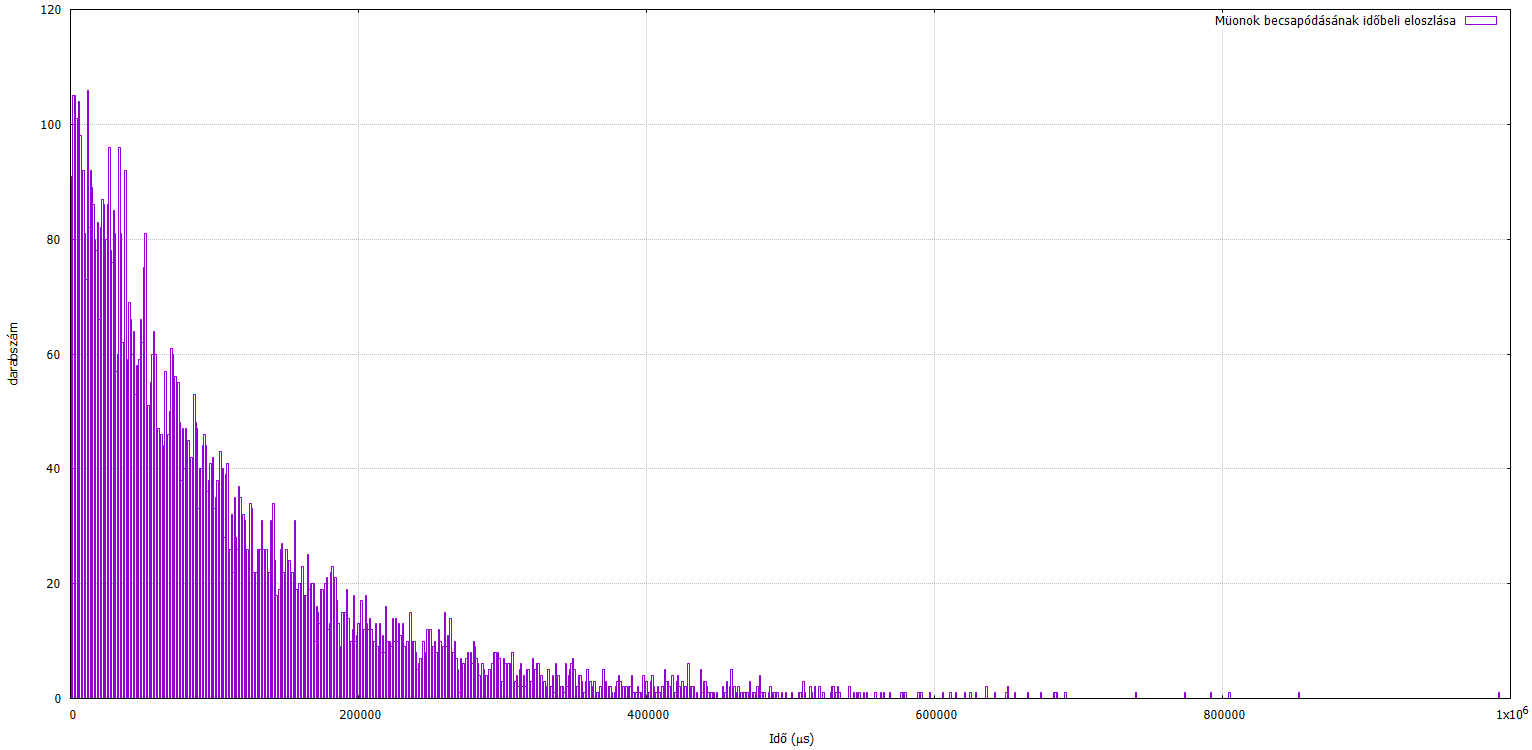
\includegraphics[width=\linewidth]{histogram1.png}}
\caption{A müonok becsapódásának ábrázolása egy kisebb binméretű hisztogramon}
\end{figure}

\pagebreak
Egy nagyobb binméretű hisztogram:
\begin{figure}[h]
{\centering 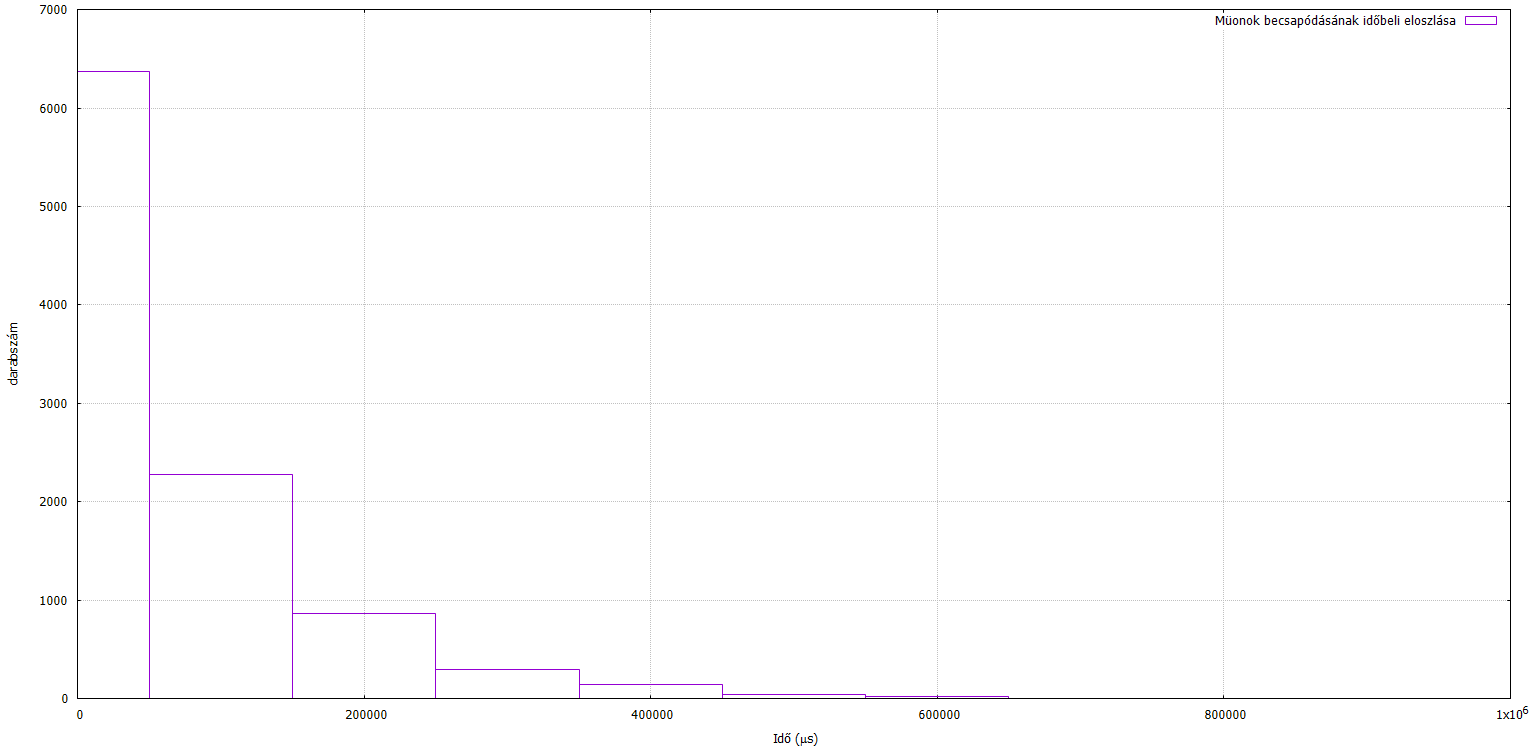
\includegraphics[width=\linewidth]{histogram2.png}}
\caption{A müonok becsapódásának ábrázolása egy nagyobb binméretű hisztogramon}
\end{figure}

Az ábrákon látszódik, hogy az eloszlás exponenciális. Ez még szembetűnőbb, ha logaritmikusan skálázzuk az első ábrát:

\begin{figure}[h]
{\centering 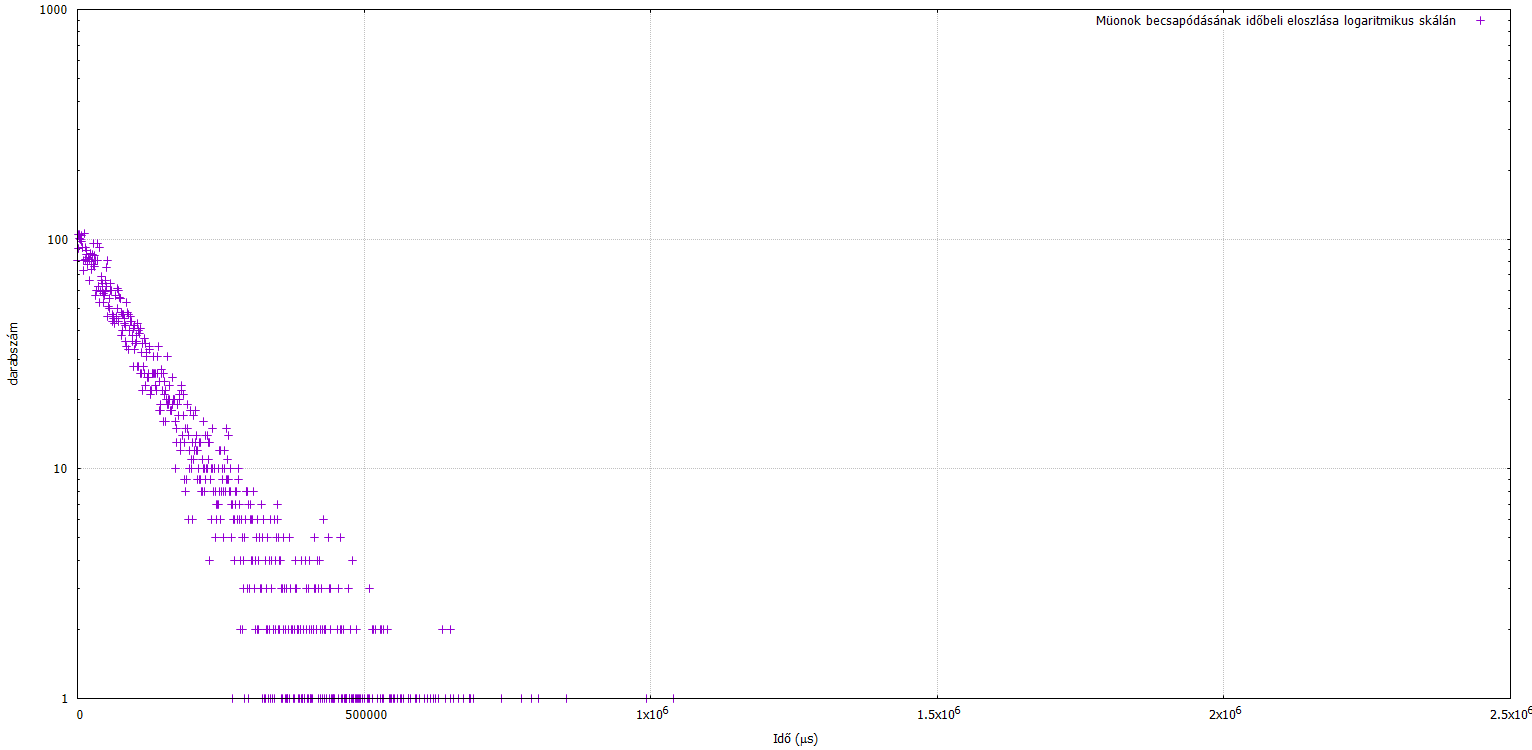
\includegraphics[width=\linewidth]{histogram3.png}}
\caption{A müonok becsapódásának ábrázolása logaritmikus skálán}
\end{figure}

A logaritmikus skálán a kisebb időértékekre jól kivehető az egyenes.




\end{document}